\documentclass[10pt,a4paper]{article}
\usepackage[utf8x]{inputenc}
\usepackage{ucs}
\usepackage{amsmath}
\usepackage{amsfonts}
\usepackage{amssymb}
\usepackage{graphicx}
\usepackage{moreverb} 
\usepackage{hyperref}
\usepackage{colortbl}
\pagestyle{headings}

\begin{document}
\renewcommand{\contentsname}{Indice} 
\renewcommand\listfigurename{Lista de Figuras}
\renewcommand\listtablename{Lista de Tablas}
\newcommand\bibname{Bibliografía}
\renewcommand{\refname}{Bibliografía}
\renewcommand\indexname{Indice alfabético}
\renewcommand\figurename{Figura}
\renewcommand\tablename{Tabla}
\renewcommand\partname{Parte}
\newcommand\chaptername{Capítulo}
\renewcommand\appendixname{Apéndice}
\renewcommand\abstractname{Resumen}

\title{Sexta semana de trabajo [12 - 16 de Mayo]}
\author{Milton Inostroza Aguilera}
\date{19 Mayo de 2008}
\clearpage
\maketitle

\begin{abstract}

Se modifica borrador de protocolo para mejor adpatación entre pyTOD y TOD:
\begin{itemize}
\item instanciación es agregado a la tabla de sucesos.
\item Se modifica por completo el registro de return.
\end{itemize}
\\
Se ha logrado solucionar los problemas que se tenían para ver el programa depurado desde la interfaz de TOD.  Se agregó, para el buen funcionamiento de la interfaz de TOD, el suceso de instanciación.

Para registrar las funciones, se ha creado una clase especial en la base de datos TOD, la cual contendrá todas las funciones que se utilicen en el lado Python.


\end{abstract}
\newpage
\tableofcontents
\newpage
\listoffigures
\newpage
\listoftables
\newpage
\section{Desarrollo}

El problema que se tenía con los timestamp era básicamente que el frame y la llamada al método/función tenían timestamp diferentes.  Se unificaron estos timestamps y se logró que la interfaz de TOD funcionara correctamente.

Las llamadas de métodos/funciones no mostraban el valor retornado por las mismas en la interfaz TOD.  Se detectó que el problema era que la profundidad debía ser depth + 1 para el registro de return y set de variables locales/atributos.

Sigue siendo necesario la modificación de la máquina virtual de Python o la creación de un tipo de datos nativo especial que permita implementar el identificador único para ver como se comporta pyTOD con este tipo de objetos.


\newpage
\section{Depuraciones}

Después de haber solucionado los problemas anteriormentes descritos, ya podemos ver la intefaz gráfica funcionando de forma más completa.\\

Se ha depurado experimentalmente el siguiente trozo de código:\\

\begin{verbatim}
class clase1(Descriptor):
    
    def __init__(self, y):
        self.x = 1
        self.c = 2
        self.z = 3
        return
    
    def metodo(self, h, i, j, k):
        self.casa = 1
        k = i + j
        return
\end{verbatim}

TOD, nos muestra la siguiente información:\\

\begin{figure}[hpb]
	\centering
	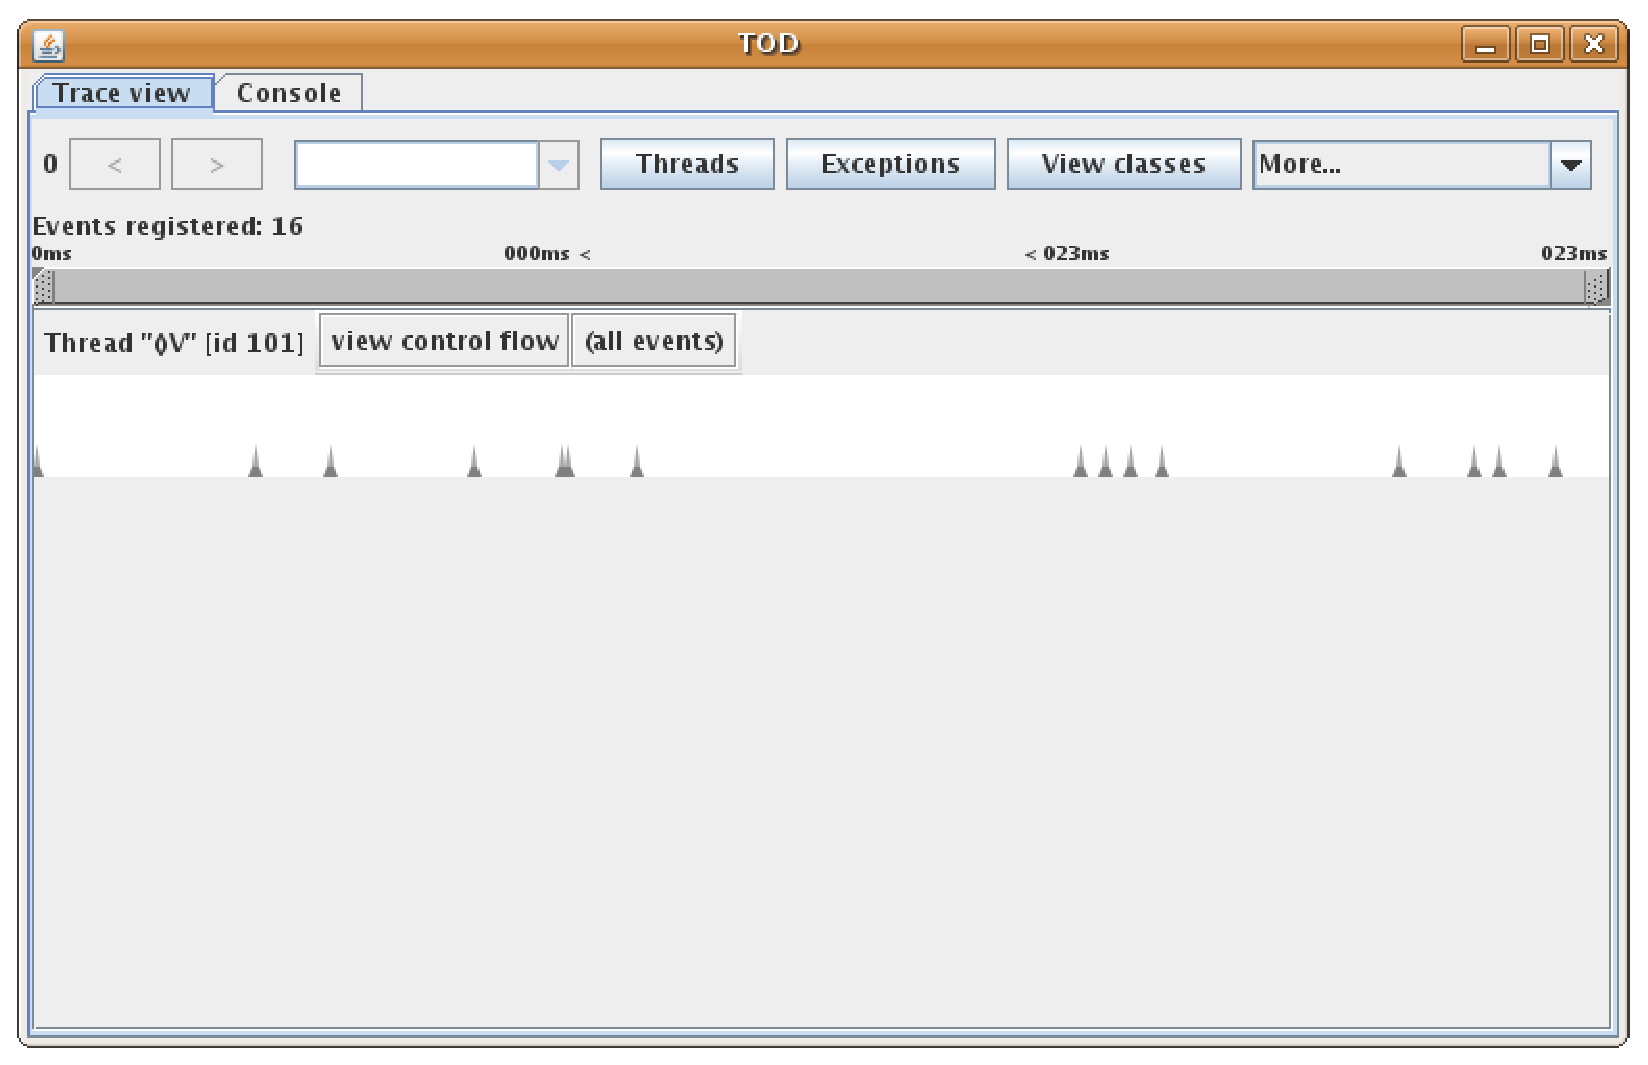
\includegraphics[scale=0.3]{images/TOD-1.eps}
	\caption{Pantalla principal de TOD}
\end{figure}

\newpage
\begin{figure}[hpb]
	\centering
	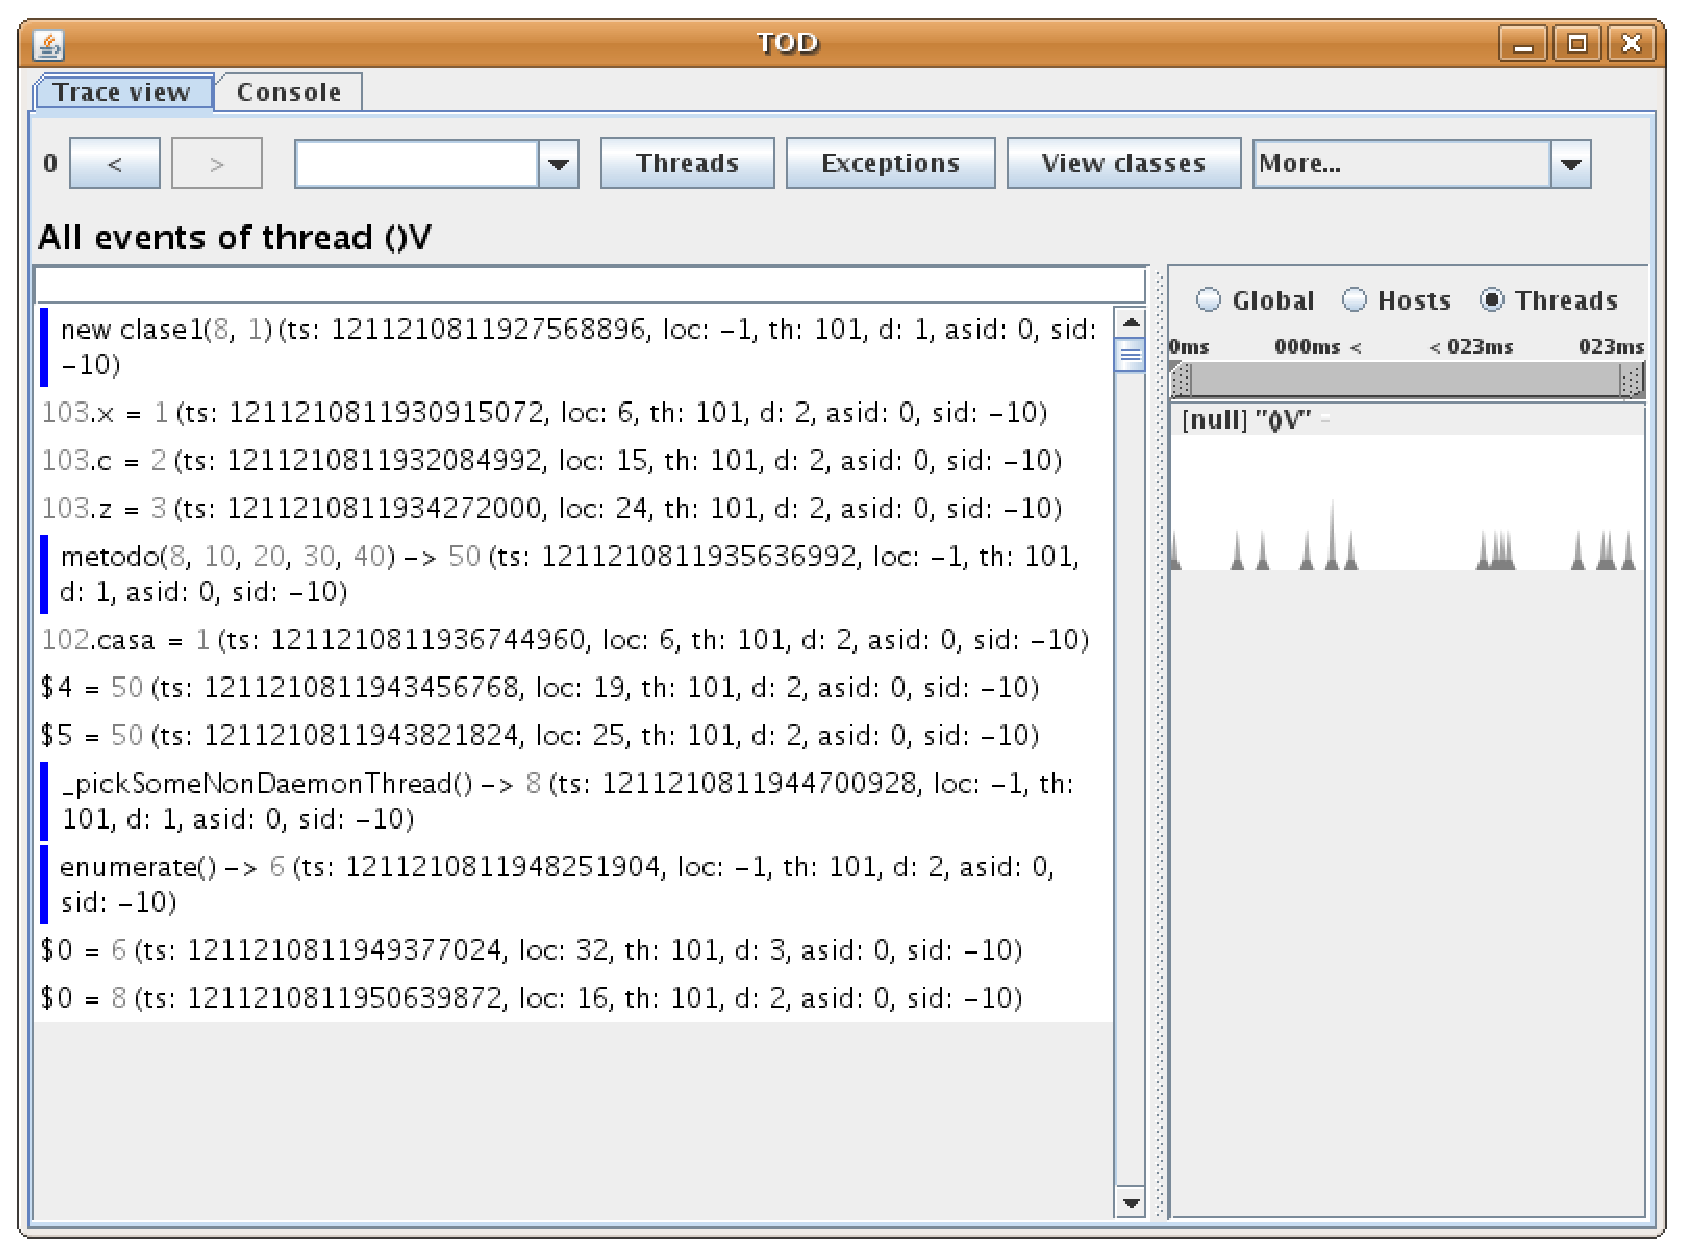
\includegraphics[scale=0.3]{images/TOD-2.eps}
	\caption{Vista de todos los eventos}
\end{figure}

\begin{figure}[hpb]
	\centering
	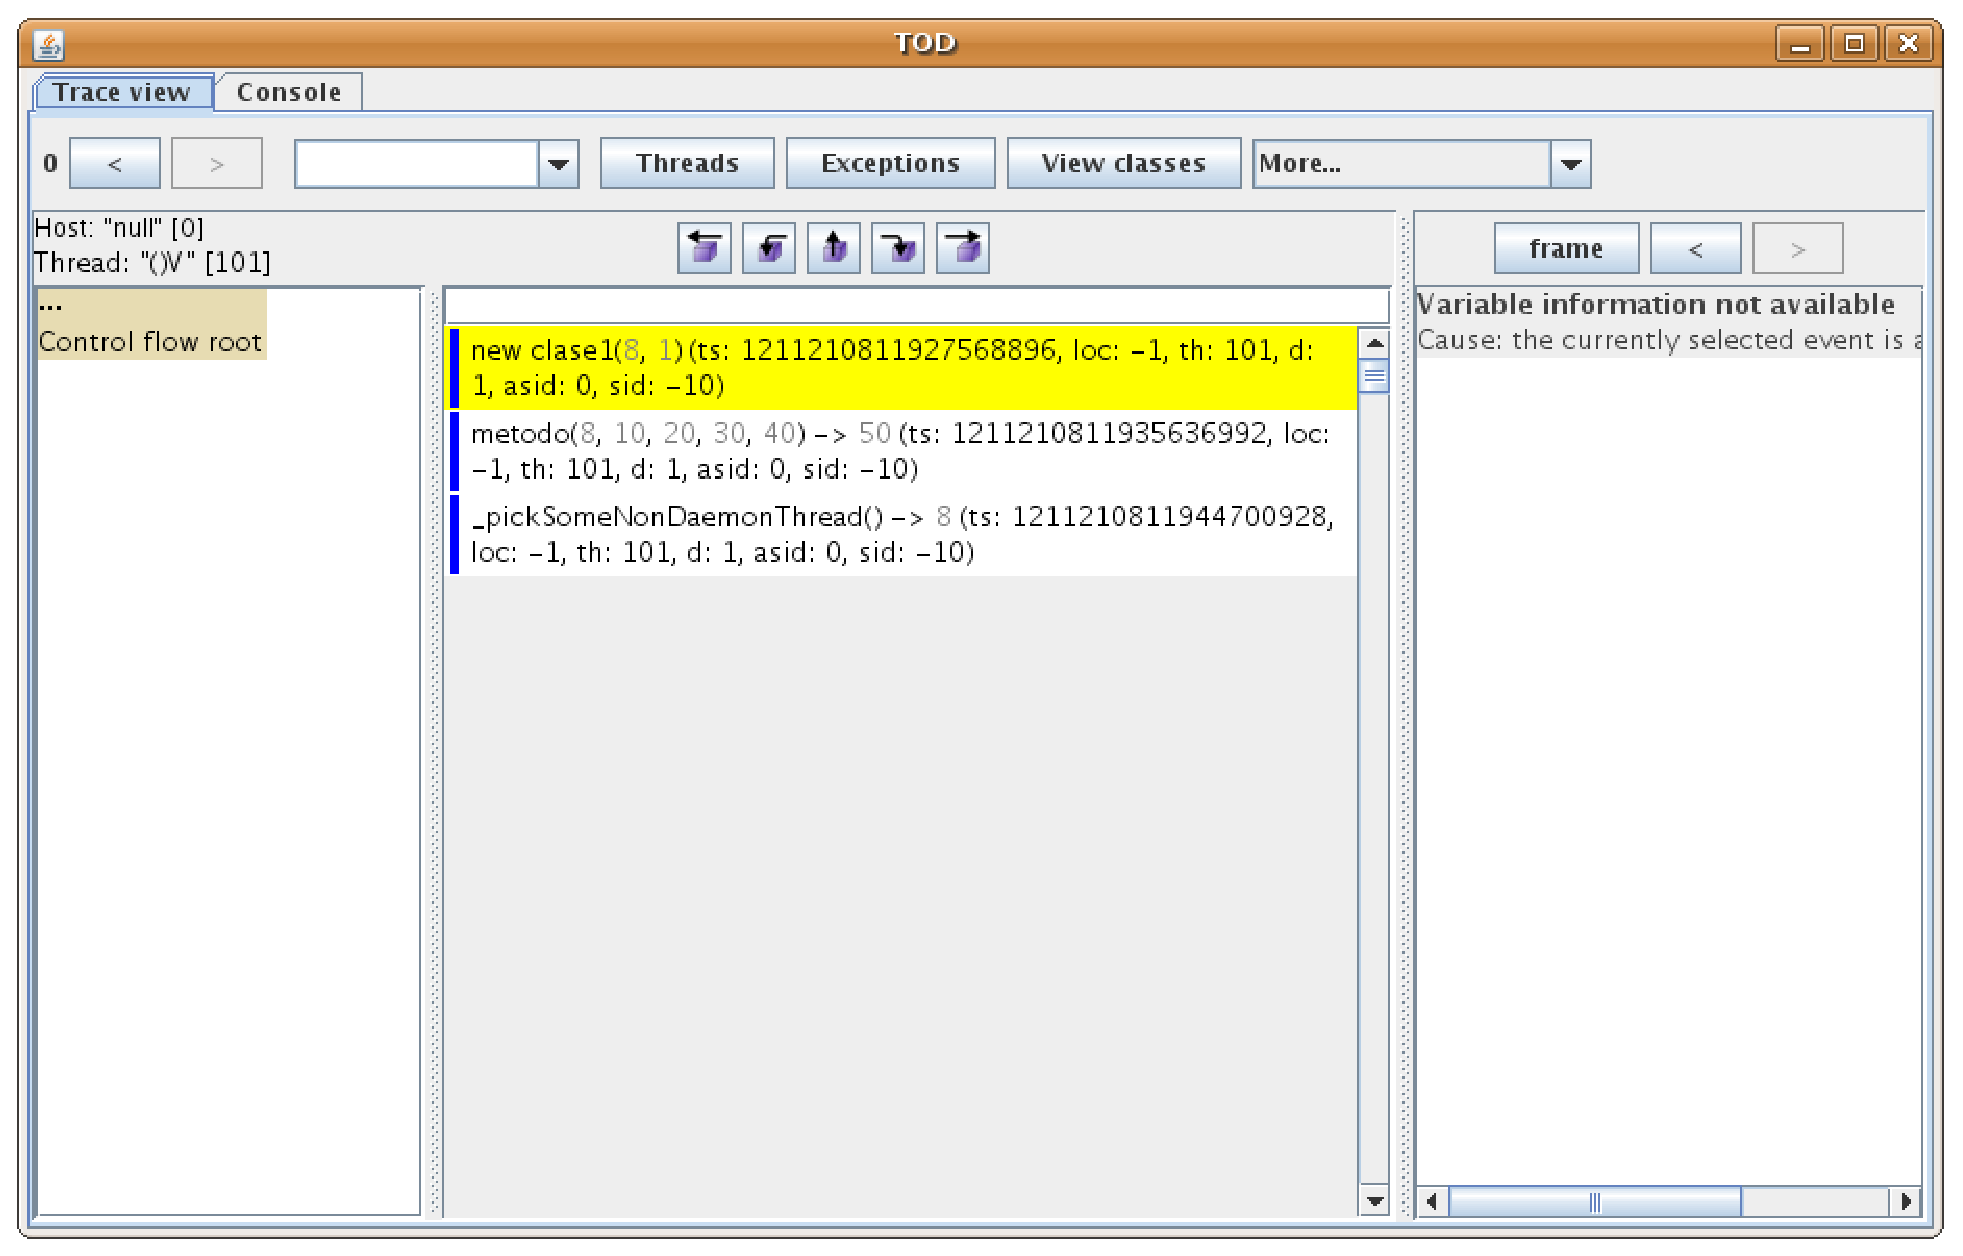
\includegraphics[scale=0.3]{images/TOD-3.eps}
	\caption{Vista del control de flujo}
\end{figure}

\newpage
\begin{figure}[hpb]
	\centering
	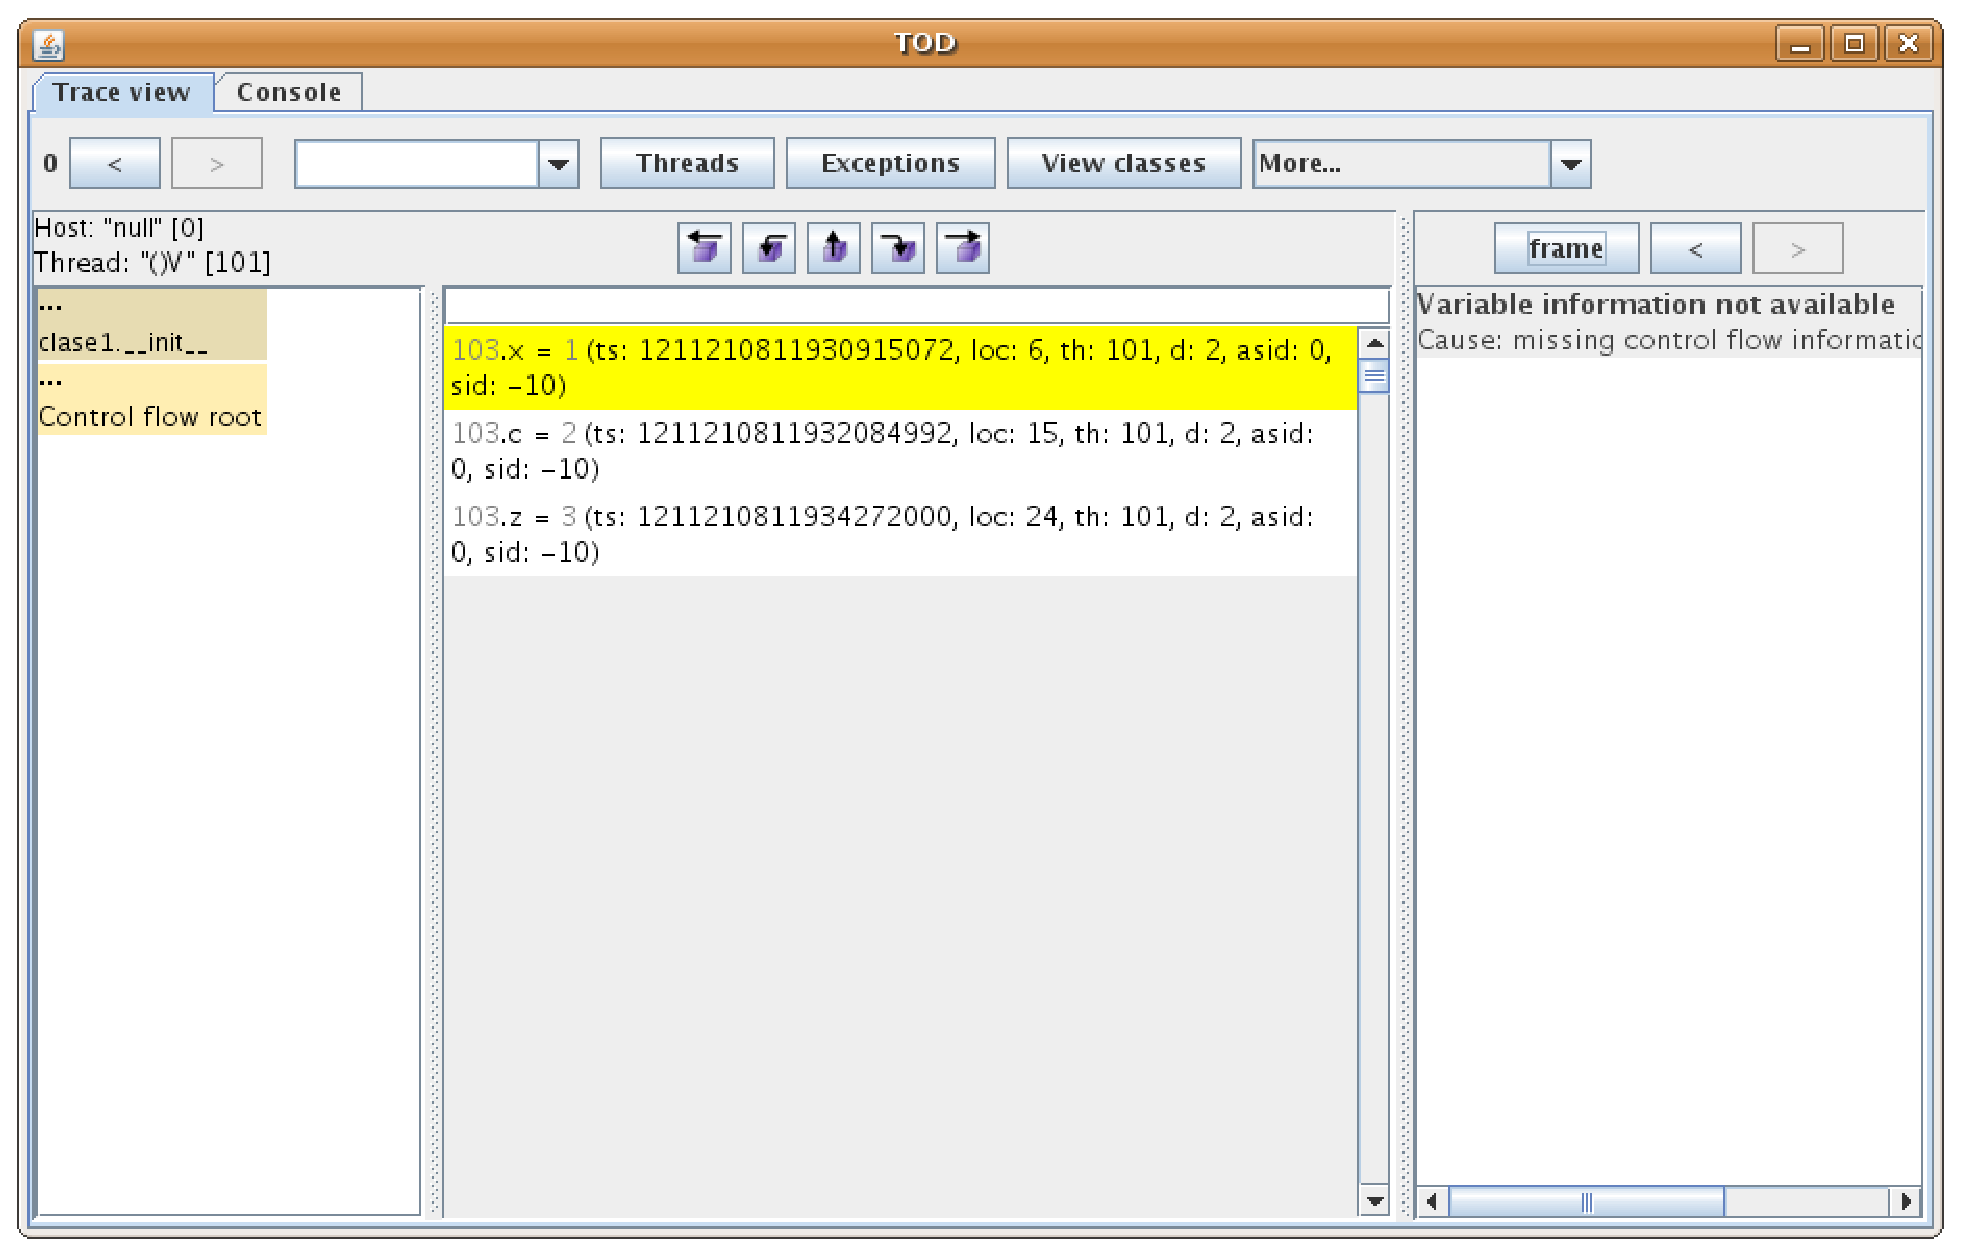
\includegraphics[scale=0.3]{images/TOD-4.eps}
	\caption{Evento instanciación seleccionado}
\end{figure}

\begin{figure}[hpb]
	\centering
	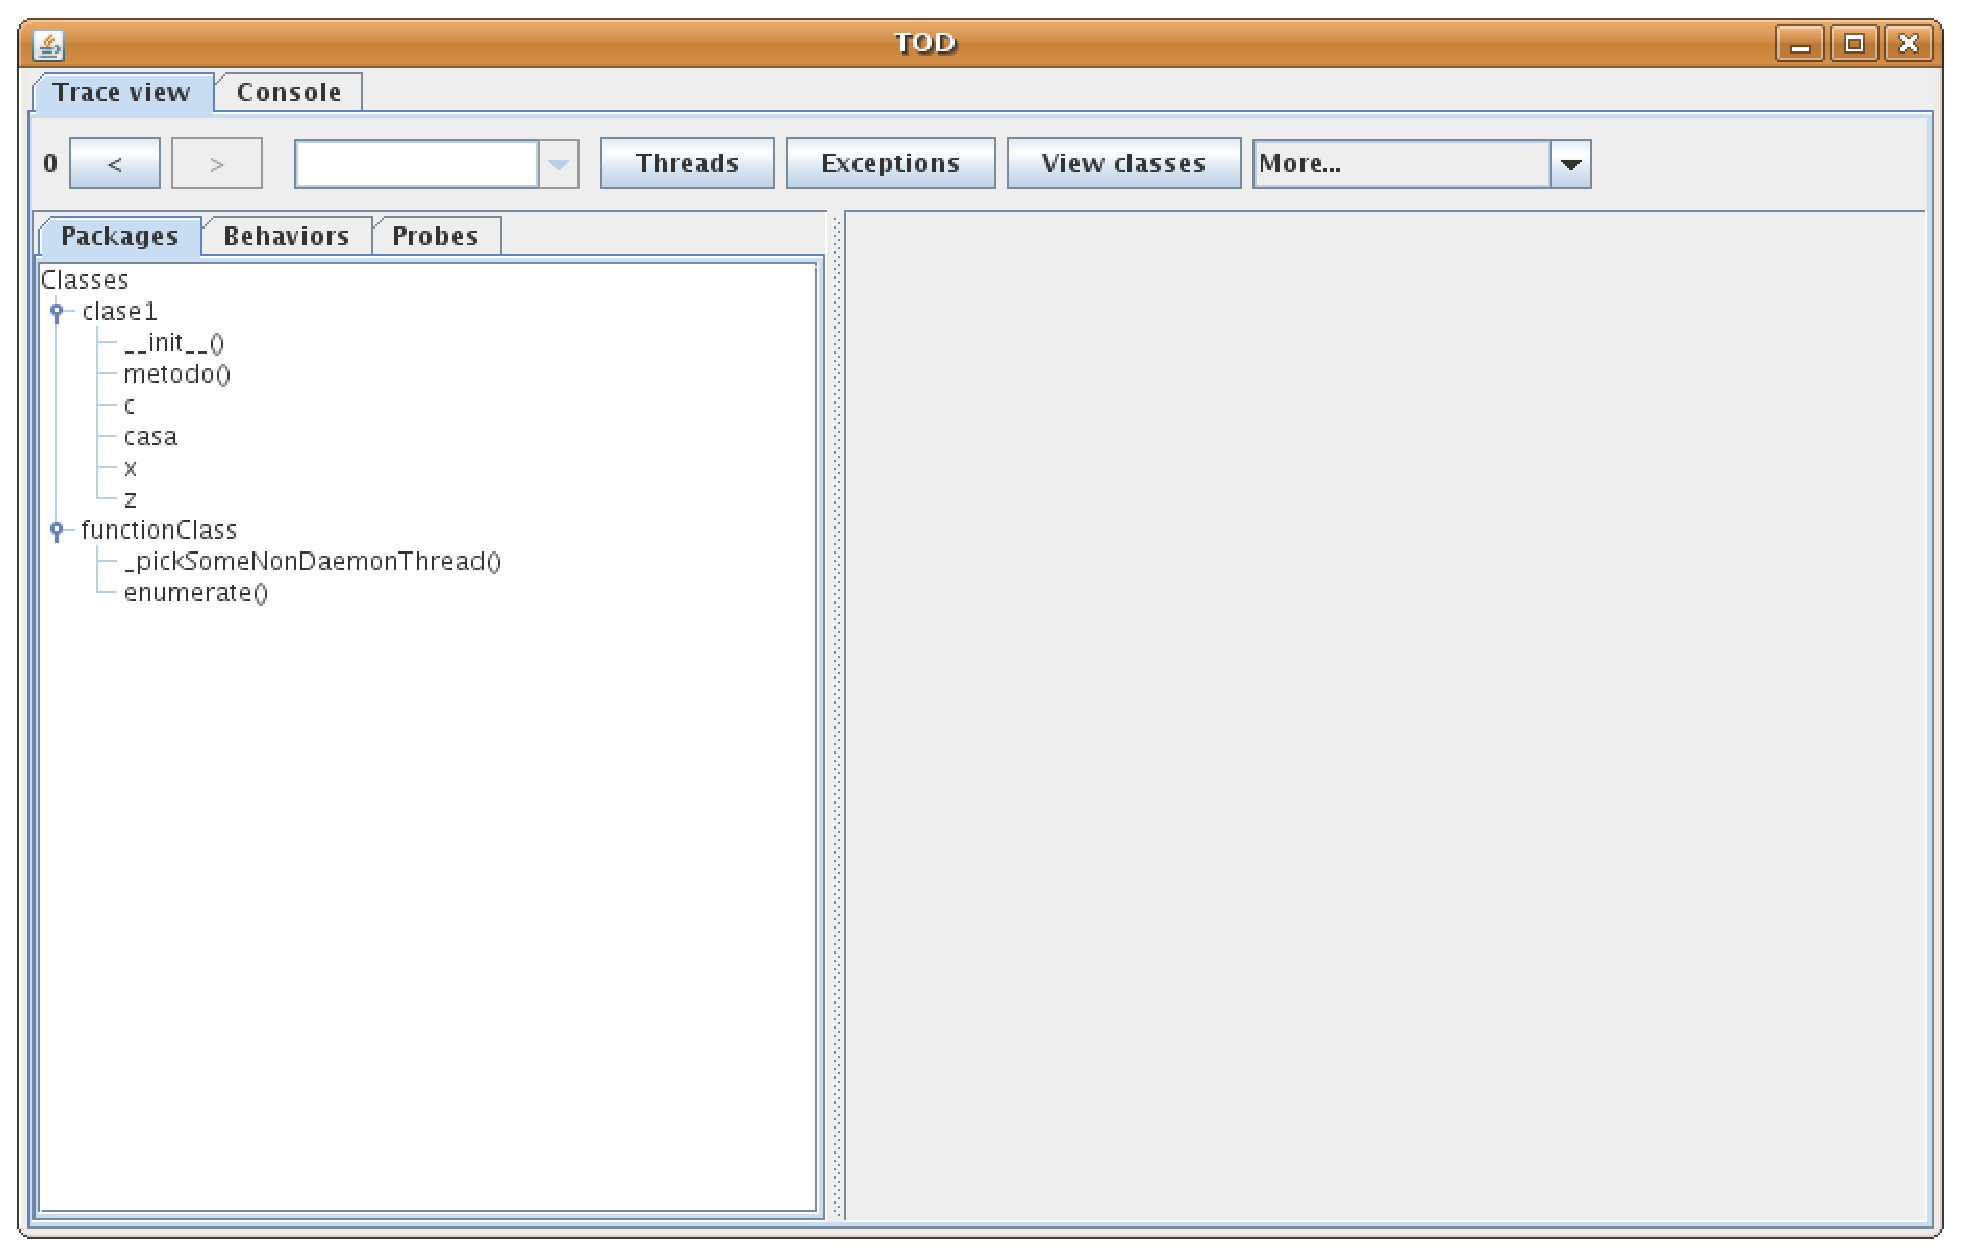
\includegraphics[scale=0.3]{images/TOD-5.eps}
	\caption{Clases, métodos y funciones}
\end{figure}

\newpage
\begin{figure}[hpb]
	\centering
	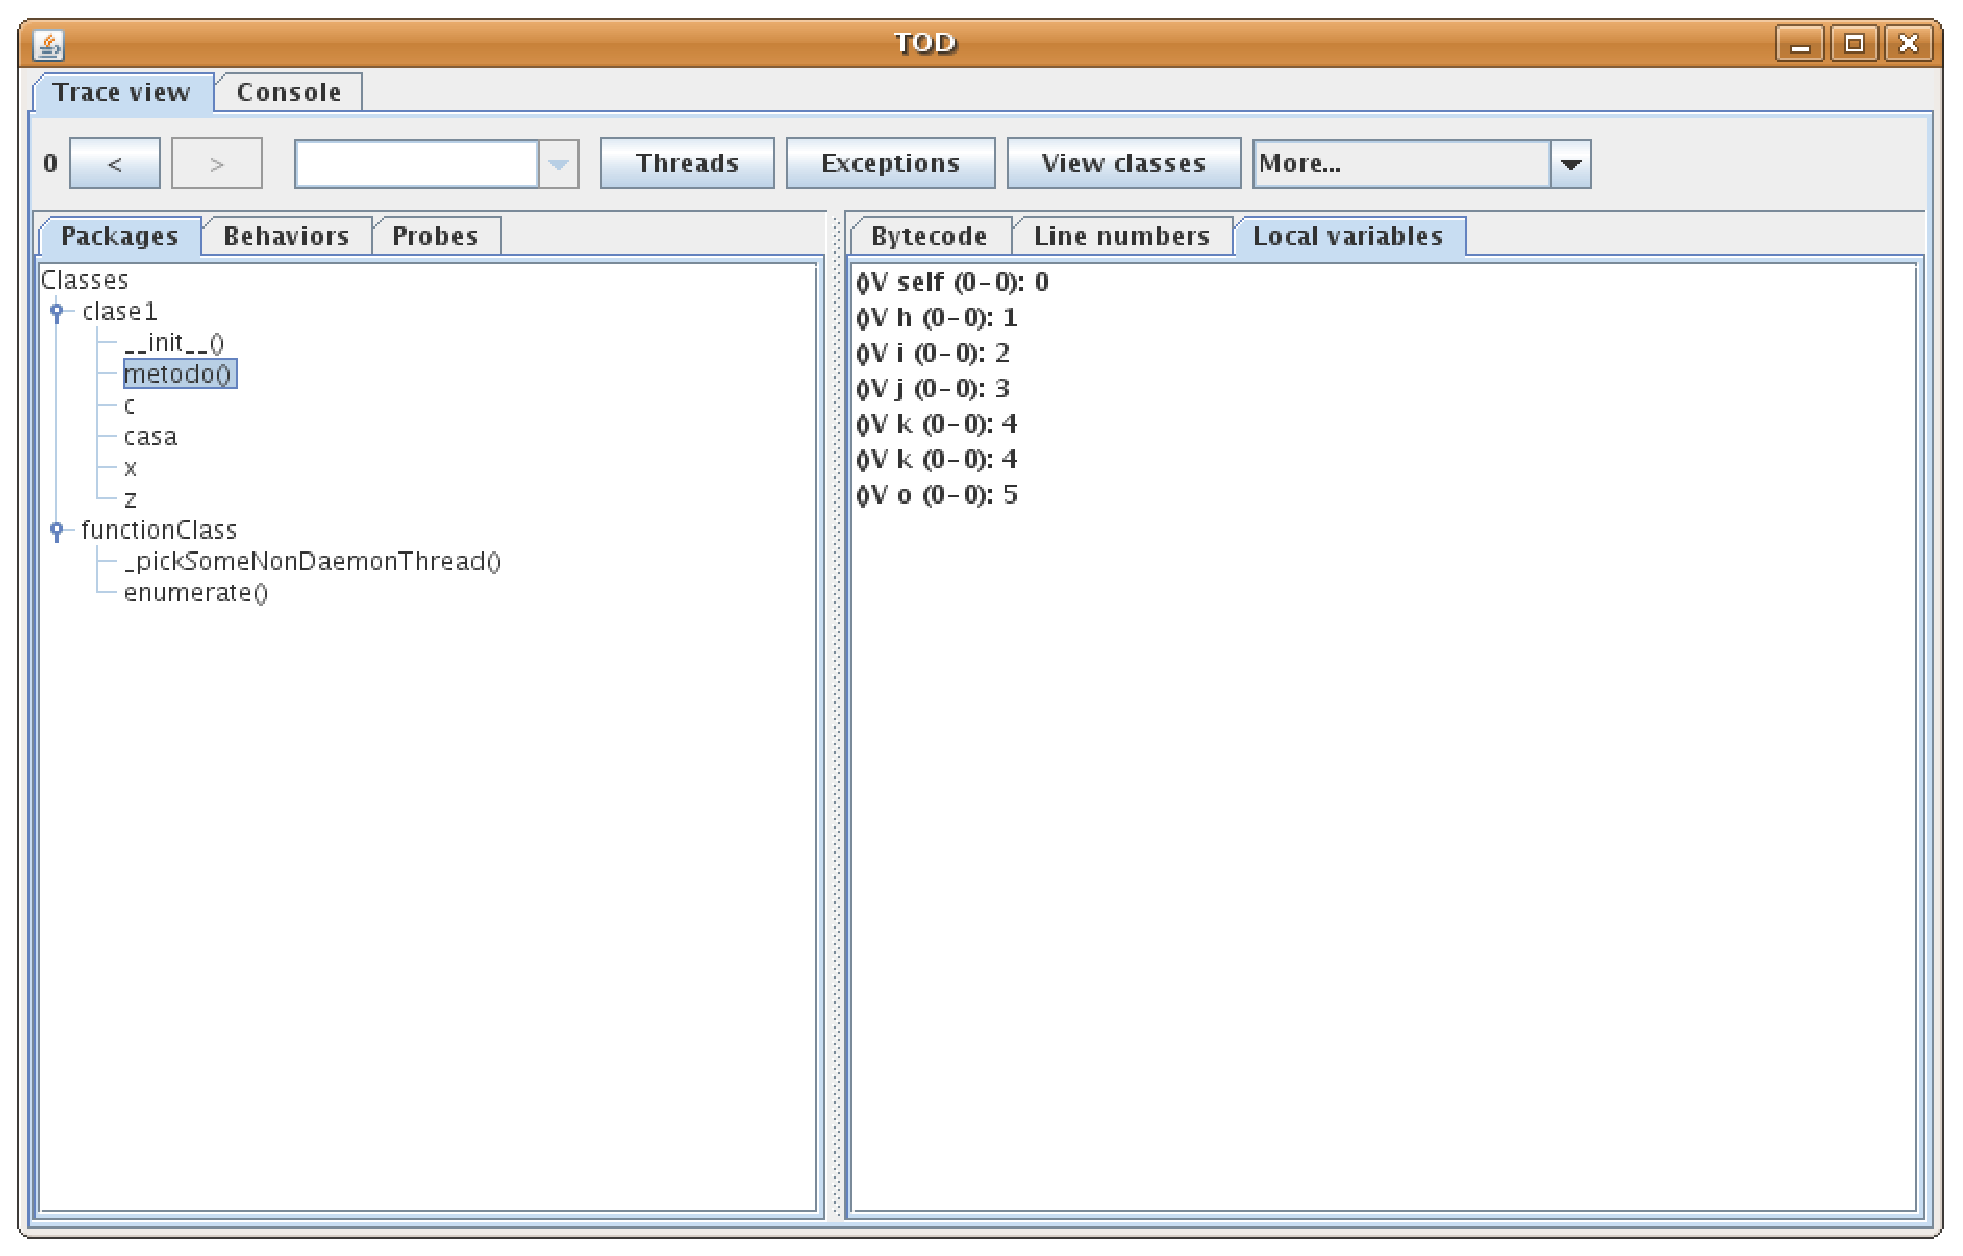
\includegraphics[scale=0.3]{images/TOD-6.eps}
	\caption{Métodos con variables locales}
\end{figure}

\begin{figure}[hpb]
	\centering
	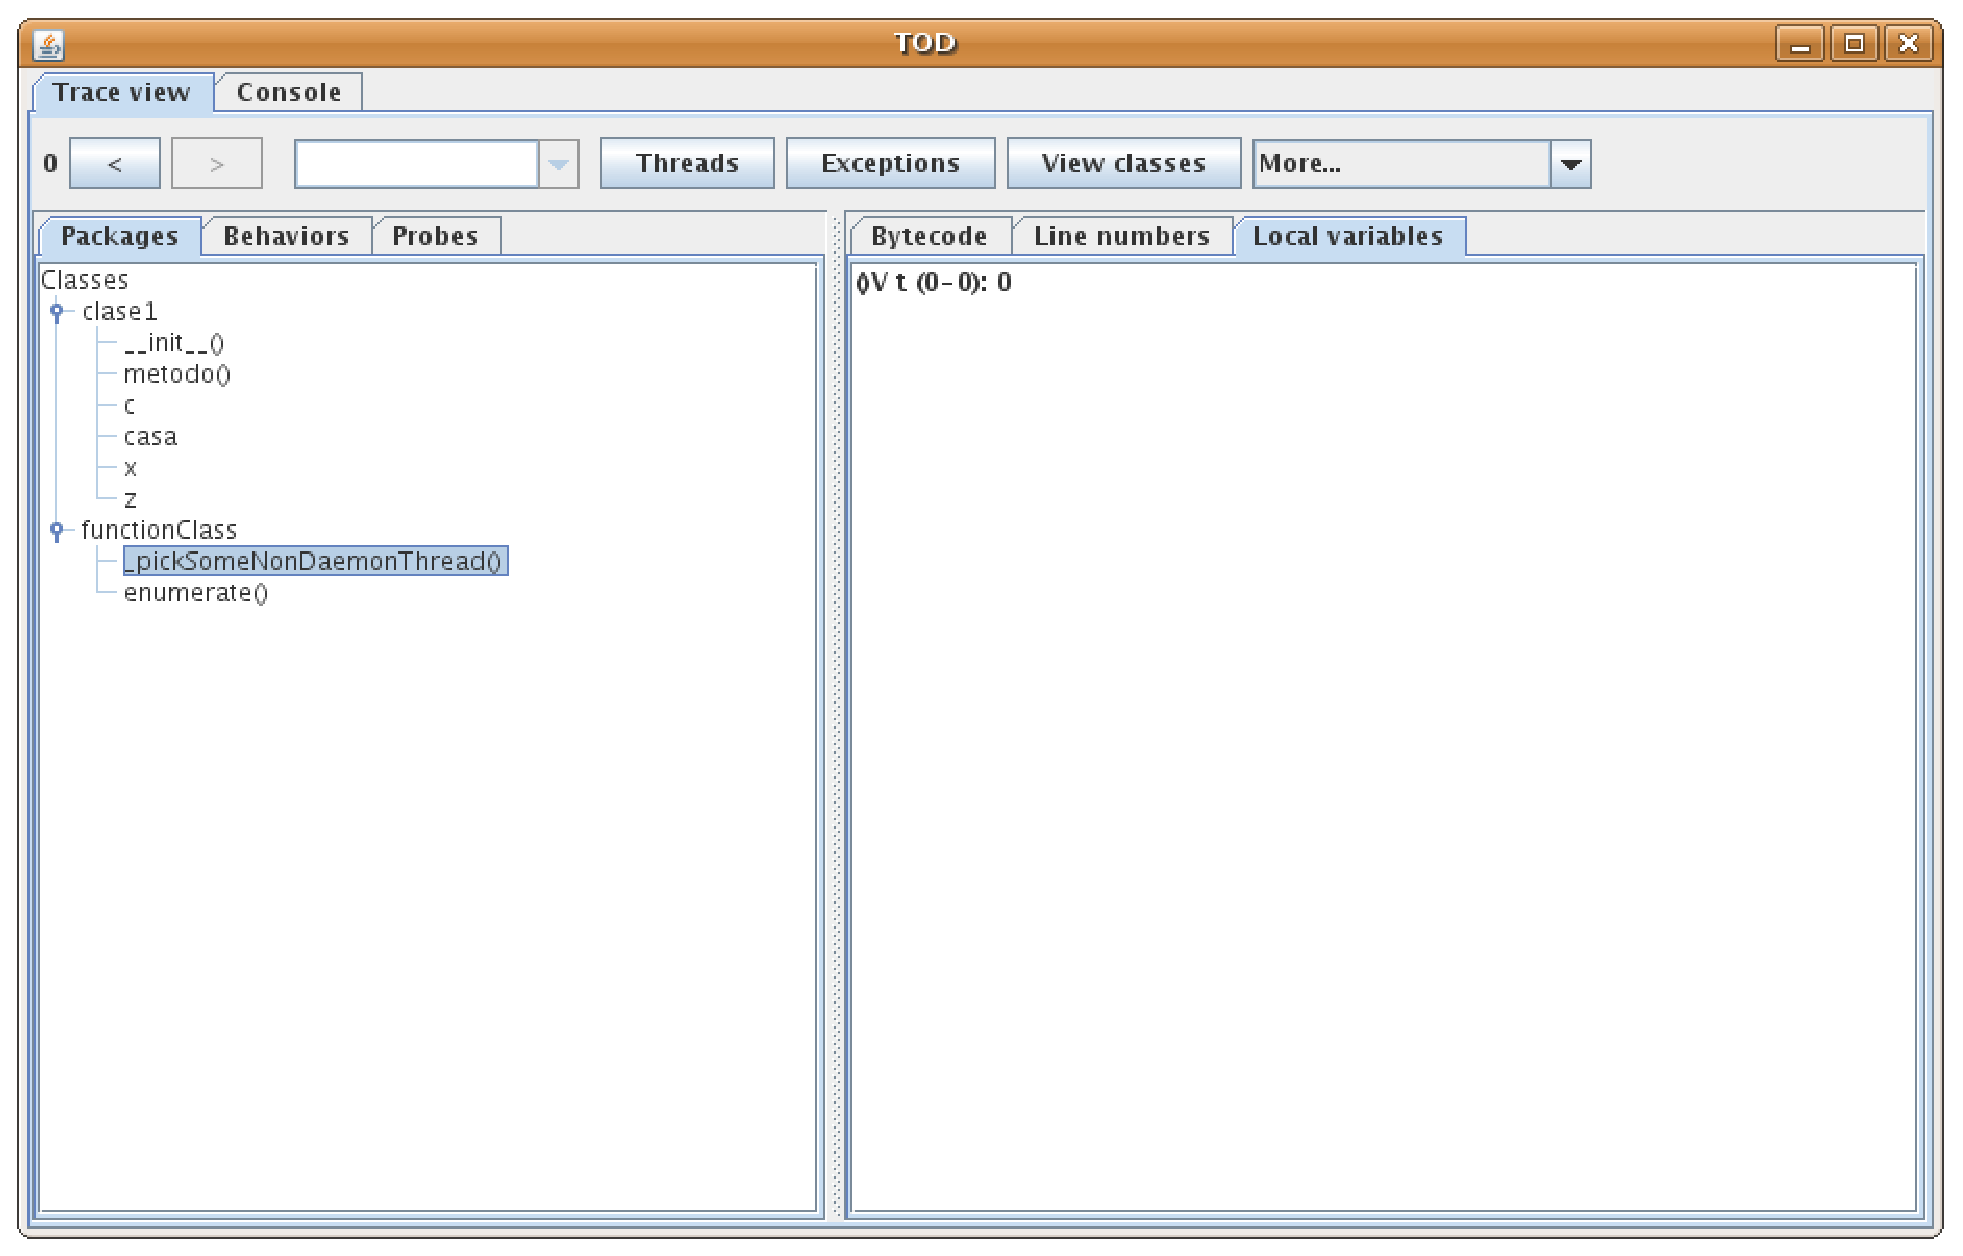
\includegraphics[scale=0.3]{images/TOD-7.eps}
	\caption{Clase para almacenar funciones}
\end{figure}

Es importante señalar que las funciones que aparecen registradas no son de nuestro código pero pertenecen a la implementación Python para el soporte de threads.


\newpage
\begin{thebibliography}{2}
\bibitem{id} \url{http://docs.python.org/lib/built-in-funcs.html}
\bibitem{howto} \url{http://docs.python.org/ext/ext.html}
\end{thebibliography}
\end{document}
